\usepackage[a4paper, margin=1in]{geometry}
\documentclass[11pt]{article}
% use UTF8 encoding
\usepackage[utf8]{inputenc}
% use KoTeX package for Korean
\usepackage[hangulfontspec, nohangul]{kotex}

\usepackage{glossaries}
\usepackage{graphicx}
\usepackage{titling}

\usepackage{amsmath}

\makeglossaries
\newacronym{cstr}{CSTR}{Continuous Stirred Tank Reactor}
\newacronym{rl}{RL}{Reinforcement Learning}
\newacronym{dqn}{DQN}{Deep Q-Network}
\newacronym{ppo}{PPO}{Proximal Policy Optimization}
\newacronym{ddpg}{DDPG}{Deep Deterministic Policy Gradient}


\begin{document}

\title{Nonlinearity를 갖는 CSTR 공정에의 RL 제어 구현 및 보상함수 변경을 통한 성능 개선}
\author{Seunghyun Cho, Hain Lee, Jaehyun Oh}
\date{\today}


\setlength{\droptitle}{-4cm}  % 제목과 페이지 상단 간격 조정
\maketitle

 
\section{Backgrounds}
\subsection{CSTR}
\gls{cstr}은 연속적으로 유체를 주입하고 동시에 반응과 혼합이 일어나는 대표적인 화학 반응기이다. 
주어진 체적 내에서 반응물이 완전히 혼합된다고 가정하며, 반응 속도, 농도 변화, 온도 제어 등 동적 특성이 중요한 시스템이다. 
특히, 비선형성(Nonlinearity)으로 인해 작은 입력 변화에도 시스템 거동이 크게 달라질 수 있어 정밀한 제어 전략이 요구된다.


\subsection{Process Control}
Process Control은 산업 공정의 안정적 운전과 최적 성능 유지를 목표로 하는 제어 공학 분야이다. 
화학, 석유화학, 제약 등의 산업에서 반응기, 증류탑, 열교환기 등 다양한 장비들의 변수(온도, 압력, 유량 등)를 제어하기 위해 활용된다. 
비선형성과 시간 지연 등 복잡한 공정 특성 때문에 전통적인 PID 제어를 넘어, 모델 예측 제어(Model Predictive Control)나 강화학습 기반 제어 방법이 연구되고 있다.



\section{목표}
Process Control의 실패는 안전성 문제로 직결될 수 있다.
CSTR 공정은 Nonlinearity 특성을 지님으로써 제어의 어려움을 유발하므로, 보다 유연하고 적응적인 제어 전략이 요구된다.\\
본 프로젝트는 Nonlinearity 특성을 지닌 \gls{cstr} 공정에 대하여 강화학습(Reinforcement Learning, RL) 기반 제어 기법을 적용하고, 이를 통해 기존 제어 방법의 한계를 극복하고자 한다.
이에 따라 본 연구에서는 심층 강화학습 알고리즘인 \gls{dqn}, \gls{ppo}, \gls{ddpg} 등을 적용하여 공정의 동적 제어를 수행하고,
\gls{cstr} 공정의 벤치마크인 Van de Vusse 반응을 통해 Reward 함수 설계에 따른 제어 성능 변화 및 공정 안정성 확보 가능성을 검증하고자 한다.


\section{Related Works}

\subsection{Library}
Bloor et al.은 Process Control의 표준 환경을 제시함으로써, Process Control 분야의 \gls{rl} 연구의 접근성을 높인 바 있다.\cite{MaximilianB2pcgym}


\subsection{Previous Researchs}
Park et al.은 CSTR의 비선형성을 고려한 보상 함수 최적화로 MPC 대비 성능을 12\% 향상시킨 바 있으며\cite{Park2024rl}, 
Yu et al.는 PPO 기반 제어 프레임워크를 통해 외란에도 불구하고 CSTR의 안정적 제어에 성공하였다.\cite{Yu2025ppo}
Bloor et al.은 강화학습과 비선형 MPC의 성능 비교를 위한 표준 환경을 제시했고\cite{bloor2024pcgym}, 
Chen et al. (1995)은 CSTR 비선형 제어 문제의 초기 벤치마크를 제공하며 후속 연구의 기반을 마련했다.\cite{chen1995benchmark}
또한 Park et al.은 Process Control에서의 \gls{rl}의 활용 연구 동향을 총망라하여, CSTR의 복잡한 동역학 제어에 유효함을 확인하였다.\cite{Park2025pc}


\section{Project Milestones}
1. PC-Gym 라이브러리의 반응식을 수정하여, Van de Vusse 반응을 묘사하고, \cite{Yu2025ppo} 에서 활용된 Tank Level을 고려대상으로 추가하여,
해당 상황에 맞는 State와 Action을 재정의한다.\\
\begin{figure}[h!]
    \centering
    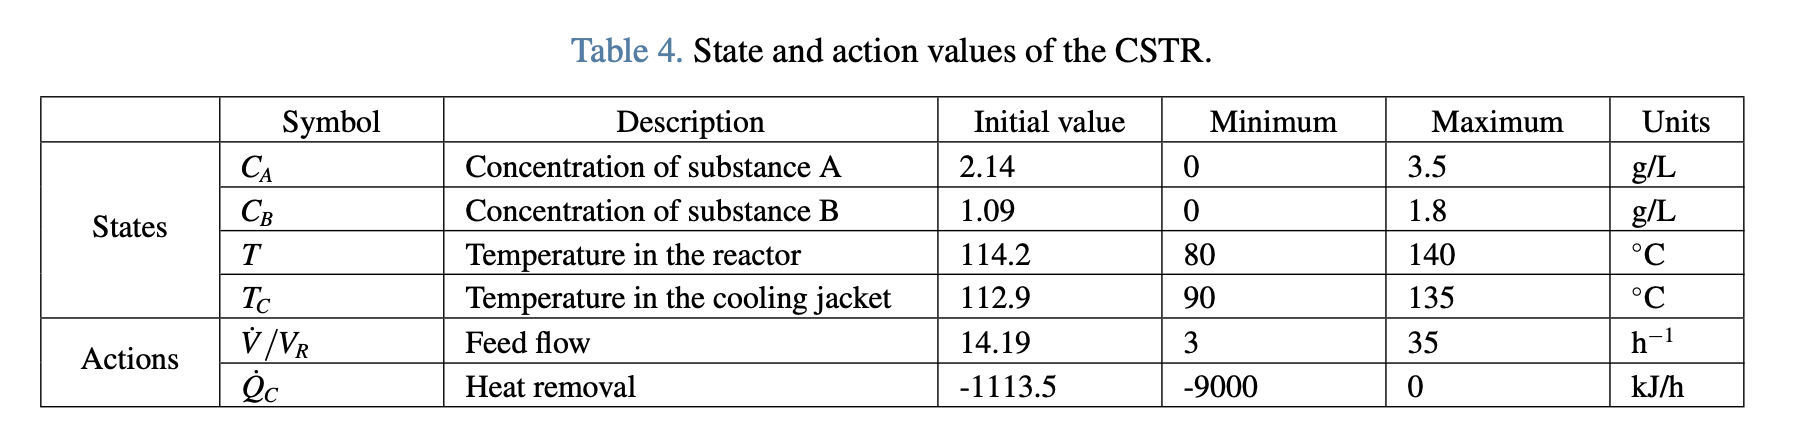
\includegraphics[width=\textwidth]{ref_table1.png} % 또는 .png, .pdf 등
    \caption{Defined states and actions in previous research}
    \label{fig1}
\end{figure}
\\
2. \gls{dqn}, \gls{ppo} 및 \gls{ddpg}를 활용하여, 각 알고리즘에 따른 베이스 모델을 구현한다.\\
3. Reward 함수를 조절하며, 세 알고리즘의 베이스모델에 대하여 벤치마크 성능을 높일 수 있는 방법을 탐색하고 이유를 공학적으로 접근하여 탐색한다.


\bibliographystyle{IEEEtran}
\bibliography{references}


\end{document}
